\documentclass[final,t]{beamer}
\mode<presentation>
{
%  \usetheme{Warsaw}
%  \usetheme{Aachen}
%  \usetheme{Oldi6}
%  \usetheme{I6td}
  \usetheme{I6dv}
%  \usetheme{I6pd}
%  \usetheme{I6pd2}
}
% additional settings
\setbeamerfont{itemize}{size=\normalsize}
\setbeamerfont{itemize/enumerate body}{size=\normalsize}
\setbeamerfont{itemize/enumerate subbody}{size=\normalsize}
\newcommand{\danielsize}{\fontsize{90}{85}\selectfont}
\newcommand{\davidsize}{\fontsize{88}{85}\selectfont}
\newcommand{\mikesize}{\fontsize{84}{85}\selectfont}

% additional packages
\usepackage{times}
\usepackage{amsmath,amsthm, amssymb, latexsym}
\usepackage{exscale}
\usepackage{multirow}
%\boldmath
\usepackage{booktabs, array}
%\usepackage{rotating} %sideways environment
\usepackage[english]{babel}
\usepackage[latin1]{inputenc}
\usepackage[orientation=landscape,size=custom,width=300,height=200,scale=2.6]{beamerposter}
\listfiles
\graphicspath{{figures/}}
% Display a grid to help align images
%\beamertemplategridbackground[1cm]

\title{\huge Unsupervised Automatic Spike Sorting} 
\author{\danielsize{Daniel Sommerman}, \davidsize{David Brody}, \mikesize{Michael Gummelt}}
\institute[Stanford University]{Department of Computer Science,
  Stanford University, Stanford, California}
\date[Dec. 14 , 2011]{Dec. 14 , 2011}

% abbreviations
\usepackage{xspace}
\makeatletter
\DeclareRobustCommand\onedot{\futurelet\@let@token\@onedot}
\def\@onedot{\ifx\@let@token.\else.\null\fi\xspace}
\def\eg{{e.g}\onedot} \def\Eg{{E.g}\onedot}
\def\ie{{i.e}\onedot} \def\Ie{{I.e}\onedot}
\def\cf{{c.f}\onedot} \def\Cf{{C.f}\onedot}
\def\etc{{etc}\onedot}
\def\vs{{vs}\onedot}
\def\wrt{w.r.t\onedot}
\def\dof{d.o.f\onedot}
\def\etal{{et al}\onedot}
\makeatother

\newcommand{\comment}[1]{}

%%%%%%%%%%%%%%%%%%%%%%%%%%%%%%%%%%%%%%%%%%%%%%%%%%%%%%%%%%%%%%%%%%%%%%%%%%%%%%%%%%%%%%%%%%%%%%%%%%%%%%%%%%%%
%%%%%%%%%%%%%%%%%%%%%%%%%%%%%%%%%%%%%%%%%%%%%%%%%%%%%%%%%%%%%%%%%%%%%%%%%%%%%%%%%%%%%%%%%%%%%%%%%%%%%%%%%%%%
\begin{document}
\begin{frame}{} 
  \begin{columns}[t]
    \begin{column}{.3\linewidth}

      %%%%%%%%%%%%%%%%%%%%%%%%%%%%%%%%%%%%%%%%%%%%%%%%%%%%%%%%%%%%%%%%%%%%%%%%%%%%%%%%%%%%%%%%%%%%%%%%%%%%%%%%%%%%

      \begin{block}{Introduction}
        Extracellular neurophysicological data recorded from a
        microelectrode is a mixture of the responses from the many
        surrounding cells. The responses are then clustered into
        similar shaped groups which represent different cells. Our
        project aims to take this analysis step which is usually done
        manually and automate it using machine learning.
      \end{block}

      %%%%%%%%%%%%%%%%%%%%%%%%%%%%%%%%%%%%%%%%%%%%%%%%%%%%%%%%%%%%%%%%%%%%%%%%%%%%%%%%%%%%%%%%%%%%%%%%%%%%%%%%%%%%

       \begin{block}{Problem and Data Description }
        We are given extracellular recordings from 60 different
        channels. Each channel represents a data stream of voltage
        potentials at a specific microelectrode. A sample recording
        looks like the following:
        \vskip1em
         \begin{center}
           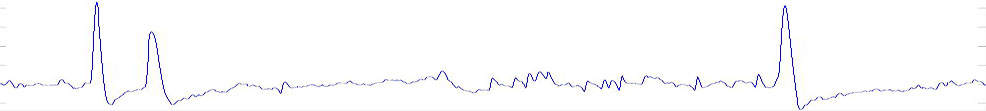
\includegraphics[width=0.8\linewidth]{images/voltagetrace_2_small.jpg}
         \end{center}
         \vskip1em
         The aim of the project is to cluster each spike into clusters
         which each share a similar shape.  Example cluster centers
         could look like the following:
         \vskip1em
         \begin{table}[ht]
           \centering
           \begin{tabular}{c c c }
             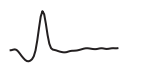
\includegraphics[width=0.2\linewidth]{images/WaveShape1.png} &
             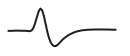
\includegraphics[width=0.2\linewidth]{images/WaveShape2.png} &
             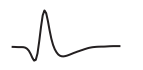
\includegraphics[width=0.2\linewidth]{images/WaveShape3.png}
           \end{tabular}
         \end{table}
         \begin{center}
         \end{center}
         \vskip1em
       \end{block}
       
       \begin{block}{Model Definitions}
          \noindent{\textbf{Model Parameters}}\par
          N = # of datapoints per channel \break
          CH = # of channels \break
          S = # of points to smooth raw data over \break
          T = Threshold for spikes \break
          L = # points to take from left of spike location
          R = # points to take from right of spike location
          \vskip1em
          \noindent{\textbf{Definitions}}\par
          We begin with the raw waveform: \break
          \begin{center}
          $R = \{ {R \in \mathbb{R}^{N x CH}; i = 1,...,CH} \}$ \break
          \end{center}
          Smoothing over S points we define a new waveform where $R^i_j$
          is the jth datapoint in the ith channel: \break
          \begin{center}
          $W^i_j = \frac{1}{s}\sum_{s=-S/2}^{S/2}R^{(i)}_{j+s}$ \break
          \end{center}
          \break
          We then define $W'$ as the zero mean normalized to the standard
          deviation on each channel of $W$. The next step is to
          separate out the possible spikes to cluster. We define the
          spike locations of interest as:
          \break
          \begin{center}
          $P = \{ i; \frac{\partial}{\partial W} = 0 \cap 
          (W_1'(P_i) > T \cup ... \cup W_{CH}'(P_i) > T) \cap i \in
          1,...,N \} $ \break
          \end{center}
          \break
          Peaks are then cut to ensure that they are a minimum of
          $\alpha = 15$ from each other. To form a single feature vector $X^{(i)}$ we take the
          surrounding points on each channel and concatentate them. \break
          \begin{center}
          $X^{(i)}_j = W'^{floor(i/(L+R+1))+1}_{mod(j, L+R+1) + P(i)}
          ; i = 1,...,|P|, j = 1,...,(L+R+1)*CH$ \break
          $X^{(i)} \in \mathbb{R}^{CH(L+R+1)}$
          \end{center}
          \break
          $X$ is the feature vector we use to then cluster on.
       \end{block}

      %%%%%%%%%%%%%%%%%%%%%%%%%%%%%%%%%%%%%%%%%%%%%%%%%%%%%%%%%%%%%%%%%%%%%%%%%%%%%%%%%%%%%%%%%%%%%%%%%%%%%%%%%%%%
      

      %%%%%%%%%%%%%%%%%%%%%%%%%%%%%%%%%%%%%%%%%%%%%%%%%%%%%%%%%%%%%%%%%%%%%%%%%%%%%%%%%%%%%%%%%%%%%%%%%%%%%%%%%%%%

    \end{column}
    \begin{column}{.3\linewidth}
      



      \begin{block}{Pipeline}
        \begin{center}
          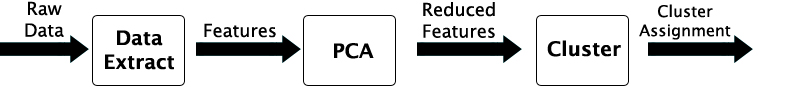
\includegraphics[width=0.8\linewidth]{images/pipeline.jpg}
        \end{center}
        
        We paramaterize our feature vectors from the raw data with the following representations:
        \begin{center}
          $X = M(R; S,T,L,R)$ 
        \end{center}
        \break
        We then use different methods to reduce the dimensionality of
        the feature vectors to improve performance and to emphasize
        more discrimanent features.
        \break
        \begin{center}
        $Red(X,N,M; X^{(i)} \in \mathbb{R}^N) = (Y^{(i)} \in
        \mathbb{R}^M,I^{(i)} \in \mathbb{R})$ 
        \break
        \end{center}
        Clustering then takes the dimension reduced feature vectors
        and assigns them to clusters which represent possible cells.
        
     \end{block}
     
     \begin{block}{Dimensionality Reduction}
       \vskip1cm
       Given the features we are now ready to perform unsupervised
       learning algorithms on the dataset. However, given the large
       size of our dataset, the running time became substantial. We
       employed various dimensionality reduction methods to help make
       the problem more tractable. Since a feature vector consists of 30 measurements for 60
channels each, we have features in $\mathbb{R}^{1800}$.
       \vskip4cm
       \noindent{\textbf{Principle Component Analysis}}

       \begin{columns}[c]
         \column{.49\linewidth}
         The first approach we took was to apply PCA to take the
         dimension of $X^{(i)}$ from $\mathbb{R}^{1800}$ to
         $\mathbb{R}^{\beta}$. Tested various $\beta$ values and found
         300 to \alert{substantially help with running time} (87\% reduction)
         without underfitting. \break \vskip1cm
         The plot on the right shows the time taken to run kmeans
         versus the dimensionality of the feature. PCA was crutial in
         rapid prototyping our clustering algorithms.
         
         \column{.48\linewidth}
         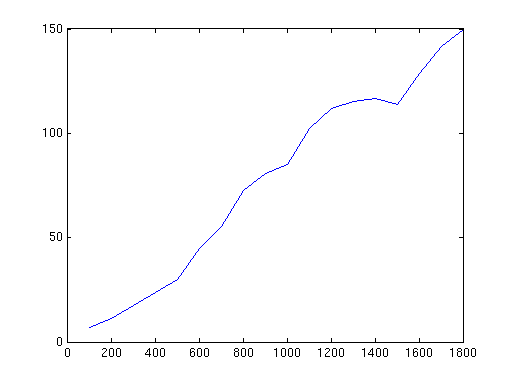
\includegraphics[width=0.97\linewidth]{images/dim_vs_runningtime.png}
       \end{columns}
       \vskip4cm
       \noindent{\textbf{Polynomial Fitting}}\par
       Another approach to reducing the dimensionality was to take
       into account the dependencies of the features within each
       channel. Since these values are continuous we can fit a
       polynomial model to them with fewer parameters. Here we let $n$
       be the number of coefficients we want to fit per channel. Since
       we have 60 channels the end result is $\mathbb{R}^{60(n+1)}$
       since the intercept parameter must be included per channel as well.
       \begin{columns}[c]
         \column{.49\linewidth}
       Our results with polynomial fitting were not as strong as
       PCA. While they do a good job of making sure each channel is
       fit well, the condensed features must encode all the
       information unlike PCA where the principle components hold the
       information. As a result, it takes many more features to get
       the same amount of information back.
       \column{.49\linewidth}
       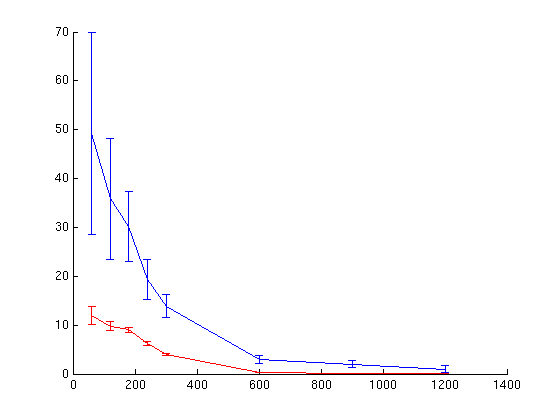
\includegraphics[width=0.97\linewidth]{images/error_poly_pca.png}
     \end{columns}
     While polynomial fitting \alert{does keep temporal information} into
     account per channel in the condensation, it \alert{fails to encode the
     meaningful information as well}.

     \end{block}
   \end{column}
   
    %%%%%%%%%%%%%%%%%%%%%%%%%%%%%%%
    
    \begin{column}{.3\linewidth}
      \begin{block}{Clustering}
        \noindent{\textbf{G-Means}}\par
        One way to choose k in the k-means algorithm is to use an algorithm
developed in 2003 by Greg Hamerly and Charles Elka, presented in the NIPS
2003 conference. In this method, a small value for k is
chosen and kmeans is run. For each cluster produced, we use a
heuristic function to decide whether to split that cluster: the
Anderson-Darling statistic. If that statistic is greater than
some threshold critical value, then we decide that the cluster should be
split. The Anderson-Darling statistic is computed as follows:
$$
A^2(Z) = -n - \frac{1}{n}\sum_{i=1}^n (2i -
1)[\log(z_i)+\log(1-z_{n+1-i})]
$$$$
A^2_*(Z) = A^2(Z)(1 + 4/n - 25/n^2)
$$
If $A^2_*(Z)$ is greater than the threshold, we split. For this
project we experimented with many thresholds and found that with $t=12$ we
got good separation between clusters.

       \begin{columns}[c,l]
         \column{.46\linewidth}
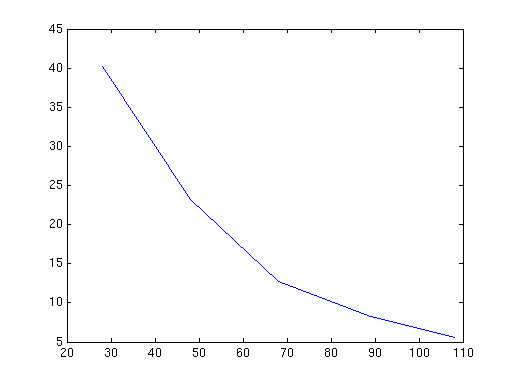
\includegraphics[width=50cm,height=26cm]{images/gmeans_k_vs_metric.png} 
         \column{.3\linewidth}
Here we plot the average Anderson-Darling statistic across all
clusters as a function of k. We can see how we arrive at a value of k
to use when the statistic crosses the threshold (6).
       \end{columns} 

       \noindent{\textbf{Davies-Bouldin Index}}\par Another way to
       determine k is via the DB Index.  It favors sets of clusters
       with high intra-cluster similarity and low inter-cluster
       similarity.  The formula is as follows:\newline


\begin{columns}[c,c]
  \column{.48\linewidth}
$X_j$ is sample $j$\\
$A_i$ is the center of cluster $i$\\
$T_i$ is the number of samples assigned to cluster $i$\newline
  \column{.48\linewidth}  
$S_i$ measures the intra cluster similarity of cluster $i$\\
$S_i = (\frac{1}{T_i} \sum\limits_{j=1}^{T_i} (X_j -
A_i)^q)^{\frac{1}{q}}$\newline
\end{columns} 


\begin{columns}[c,c]
  \column{.40\linewidth}
$M_{ij}$ measures the inter cluster similarity of clusters $i$ and $j$\\
$M_{ij} = (\sum\limits_{k=1}^{N} |a_{ki} - a{kj}|^p)^{\frac{1}{p}}$\newline

$DB$ is the Davies Bouldin index\\
$DB = \frac{1}{N} \sum\limits_{i=1}^N \max_{j:i \neq j} R_{ij}$\newline

The graph to the right is of k vs DB:\newline
  \column{.55\linewidth}  
  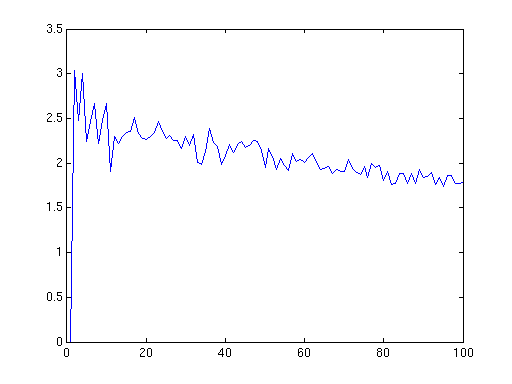
\includegraphics[width=0.97\linewidth]{images/davies_k_vs_davies_index.png}
\end{columns} 

      \end{block}

       \begin{block}{Conclusion}
        \vskip1ex
        \noindent{\textbf{Conclusions}}
        \begin{itemize}
        \item PCA was very useful for compressing the data well
        \item Understanding meaning of data and how to format it
          correctly is important
        \item The number of clusters and the confidence of them is
          very dependent on the heuristic used.
        \end{itemize}

        \vskip1ex
        \noindent{\textbf{Learnings}}
        \begin{itemize}
        \item Performing unsupervised learning with real world data is
          difficult.
          \item Choosing right heuristic for clustering is important
        \end{itemize}

        \vskip1ex
        \noindent{\textbf{Future Work}}
        \begin{itemize}
          \item Using polynomial fitting then PCA to compress
          \item Use better clustering algorithm to take specific
            neurophysiological heuristics into account.
        \end{itemize}

        \vspace{-1ex}
      \end{block}
%%%%%%%%%%%%%%%%%%%%%%%%%%%%%%%%%%%%%%%%%%%%%%%%%%%%%%%

    \end{column}
  \end{columns}
\end{frame}

\end{document}


%%%%%%%%%%%%%%%%%%%%%%%%%%%%%%%%%%%%%%%%%%%%%%%%%%%%%%%%%%%%%%%%%%%%%%%%%%%%%%%%%%%%%%%%%%%%%%%%%%%%
%%% Local Variables: 
%%% mode: latex
%%% TeX-PDF-mode: t
%%% End: 
